
%Superscripts and subscripts that are words or abbreviations, as in
%\( \pi_{\mathrm{low}} \), should be typed as roman letters; this is
%done as \verb|\( \pi_{\mathrm{low}} \)| instead of \( \pi_{low} \)
%done by \verb|\( \pi_{low} \)|.

%User-defined macros should be placed in the preamble of the chapter,
%and not at any other place in the document. Definitions made using
%the commands \verb|\newcommand,| \verb|\renewcommand,|
%\verb|\newenvironment| or \verb|\renewenvironment| should be used
\newcommand{\Br}{\ensuremath{B\!\rho}}
\newcommand{\bull}{\ensuremath{\bullet~}}
\newcommand{\Bz}{\ensuremath{{B_z}}}
\newcommand{\com}{\ensuremath{\it com}}
\newcommand{\dip}{{\it DIPOLE}}
\newcommand{\EFB}{\ensuremath{E\!F\!B}}
\newcommand{\EFBs}{\ensuremath{E\!F\!B\!s}}
\newcommand{\ffag}{{\it FFAG}}
\newcommand{\lab}{\ensuremath{lab}}
\newcommand{\MC}{Monte~Carlo}


\chapter[FFAG]{FFAG}\label{chapFFAG}


\section{Introduction}\label{secCycloIntro}

%You can obtain these files from our web pages at:
%\url{http://www.worldscientific.com/page/authors/book-stylefiles} and
%\url{http://www.icpress.co.uk/authors/stylefiles.shtml#books}.

Beyond simple knowledge and concepts, this Chapter introduces to the basic principles and formulas attached 
to the FFAG accelerators, 
which will be manipulated during the user computer exercises. 
Deeper insight in the theory and technology 
of  FFAG accelerators  
can be found in the brief series of refrences cited in this chapter. 
The candidate to the computer exercises which follow is encouraged to first read these references. 

\begin{figure}[ht]
\sidebyside
{
  \begin{minipage}{.47\linewidth}
    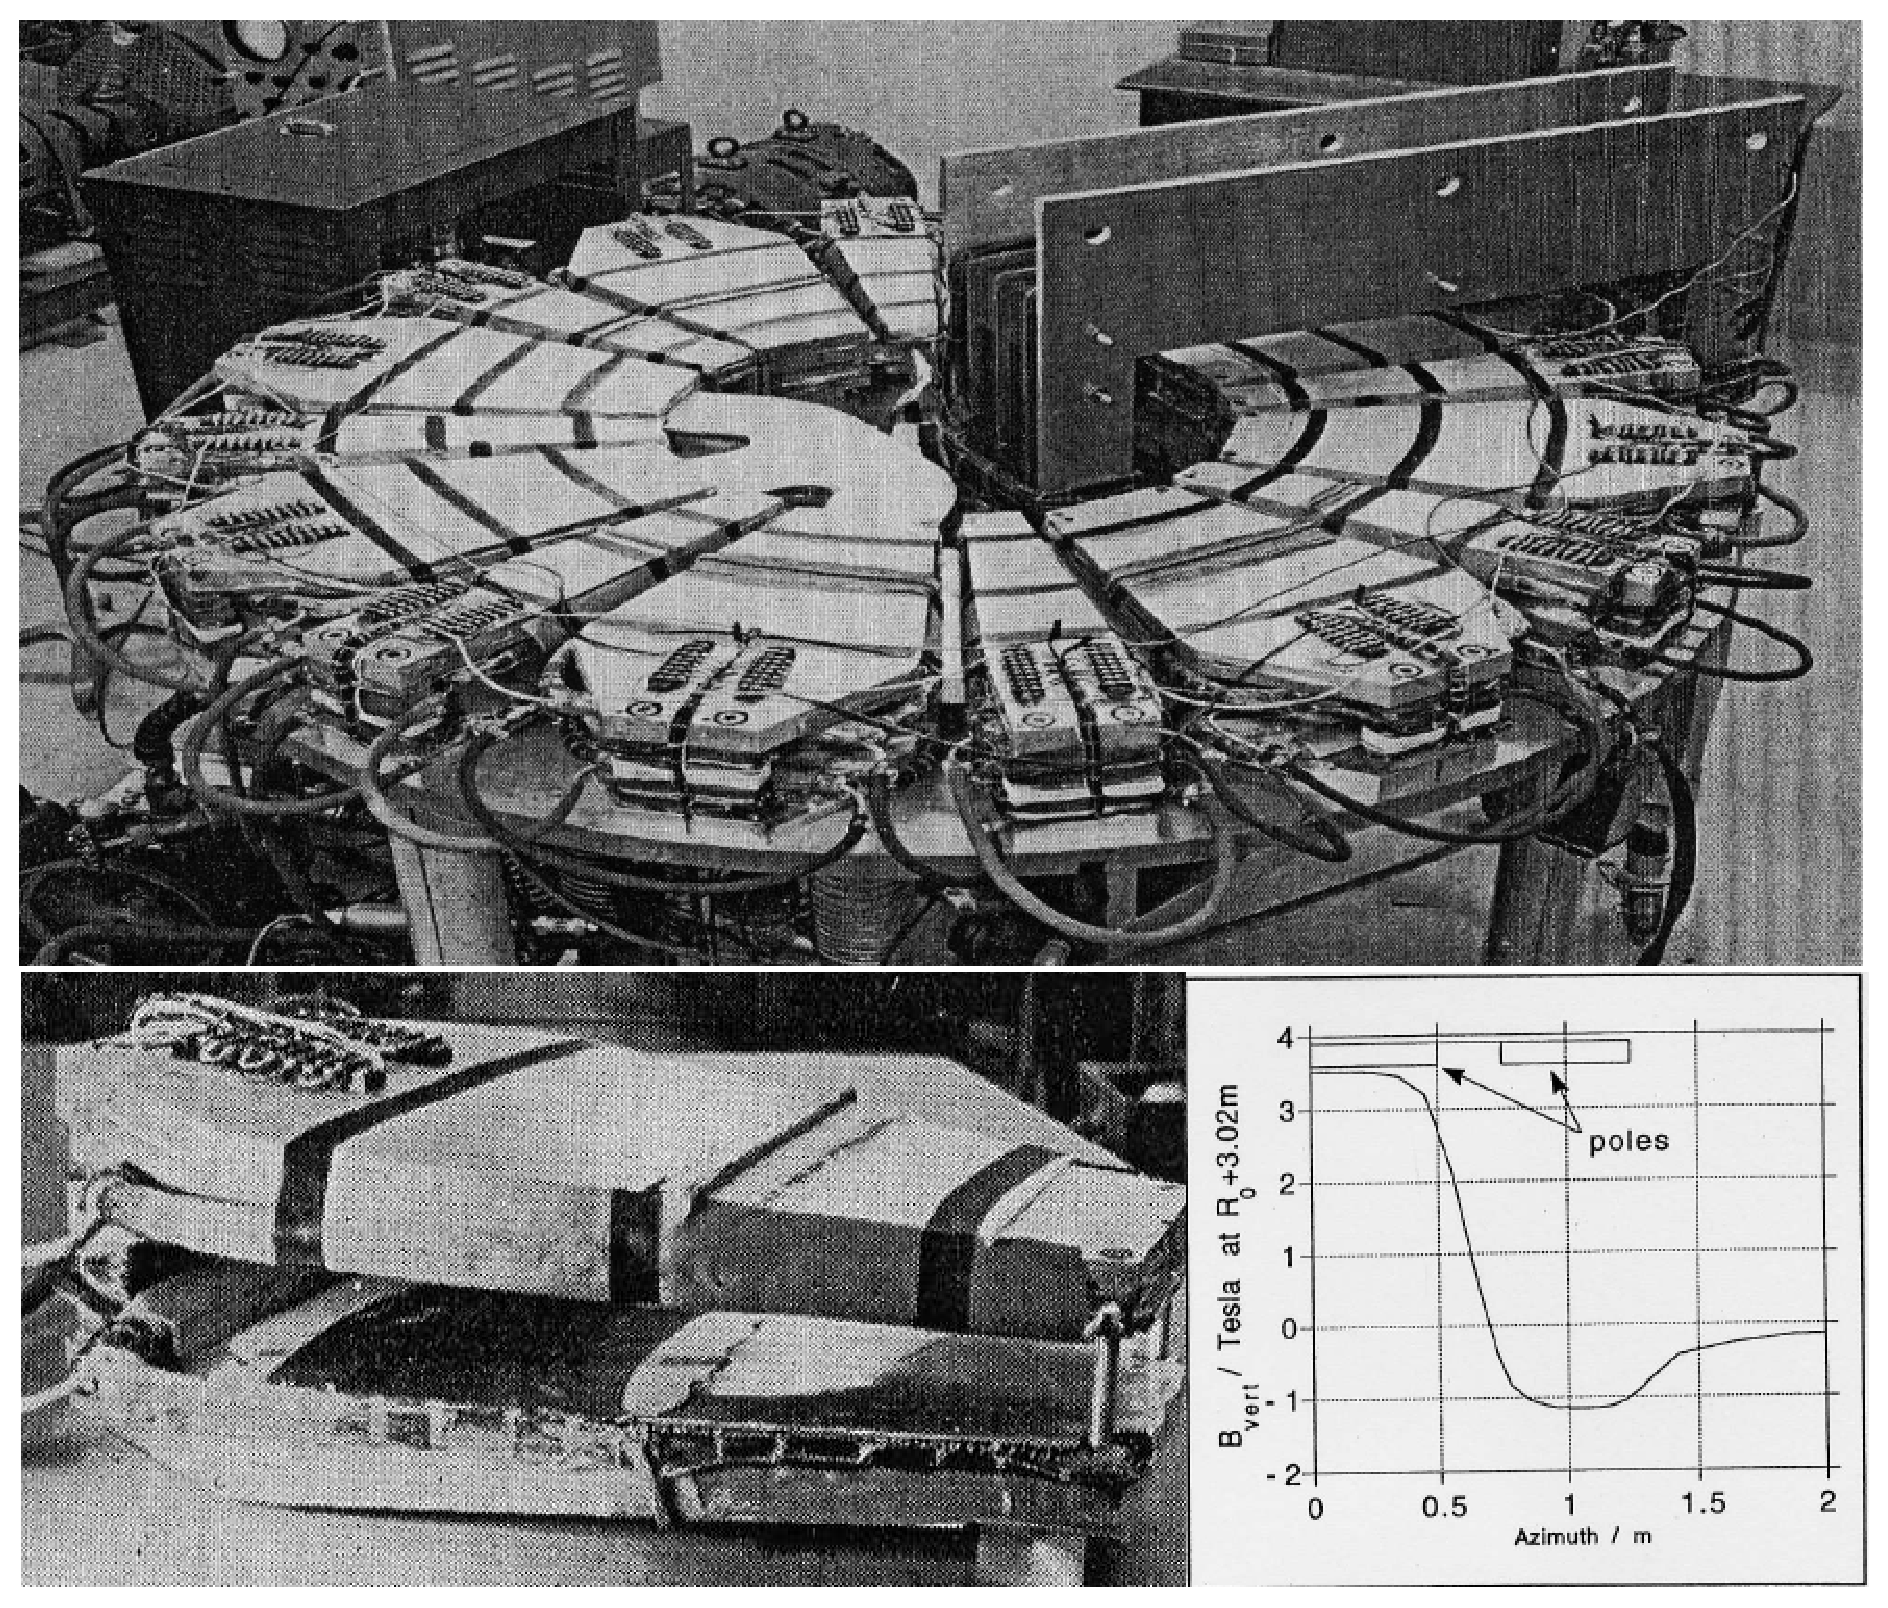
\includegraphics[width=0.99\linewidth]{./figures/MARKII.eps}
    \caption{
    MURA's MARK II and its induciton acceleration, the 
 first electron FFAG (first beam in 1956 ******)~\cite{BibFFAG-1}.
    } 
    \label{figFFAG_MARKII}
   \end{minipage}
}{
  \begin{minipage}{.45\linewidth}
    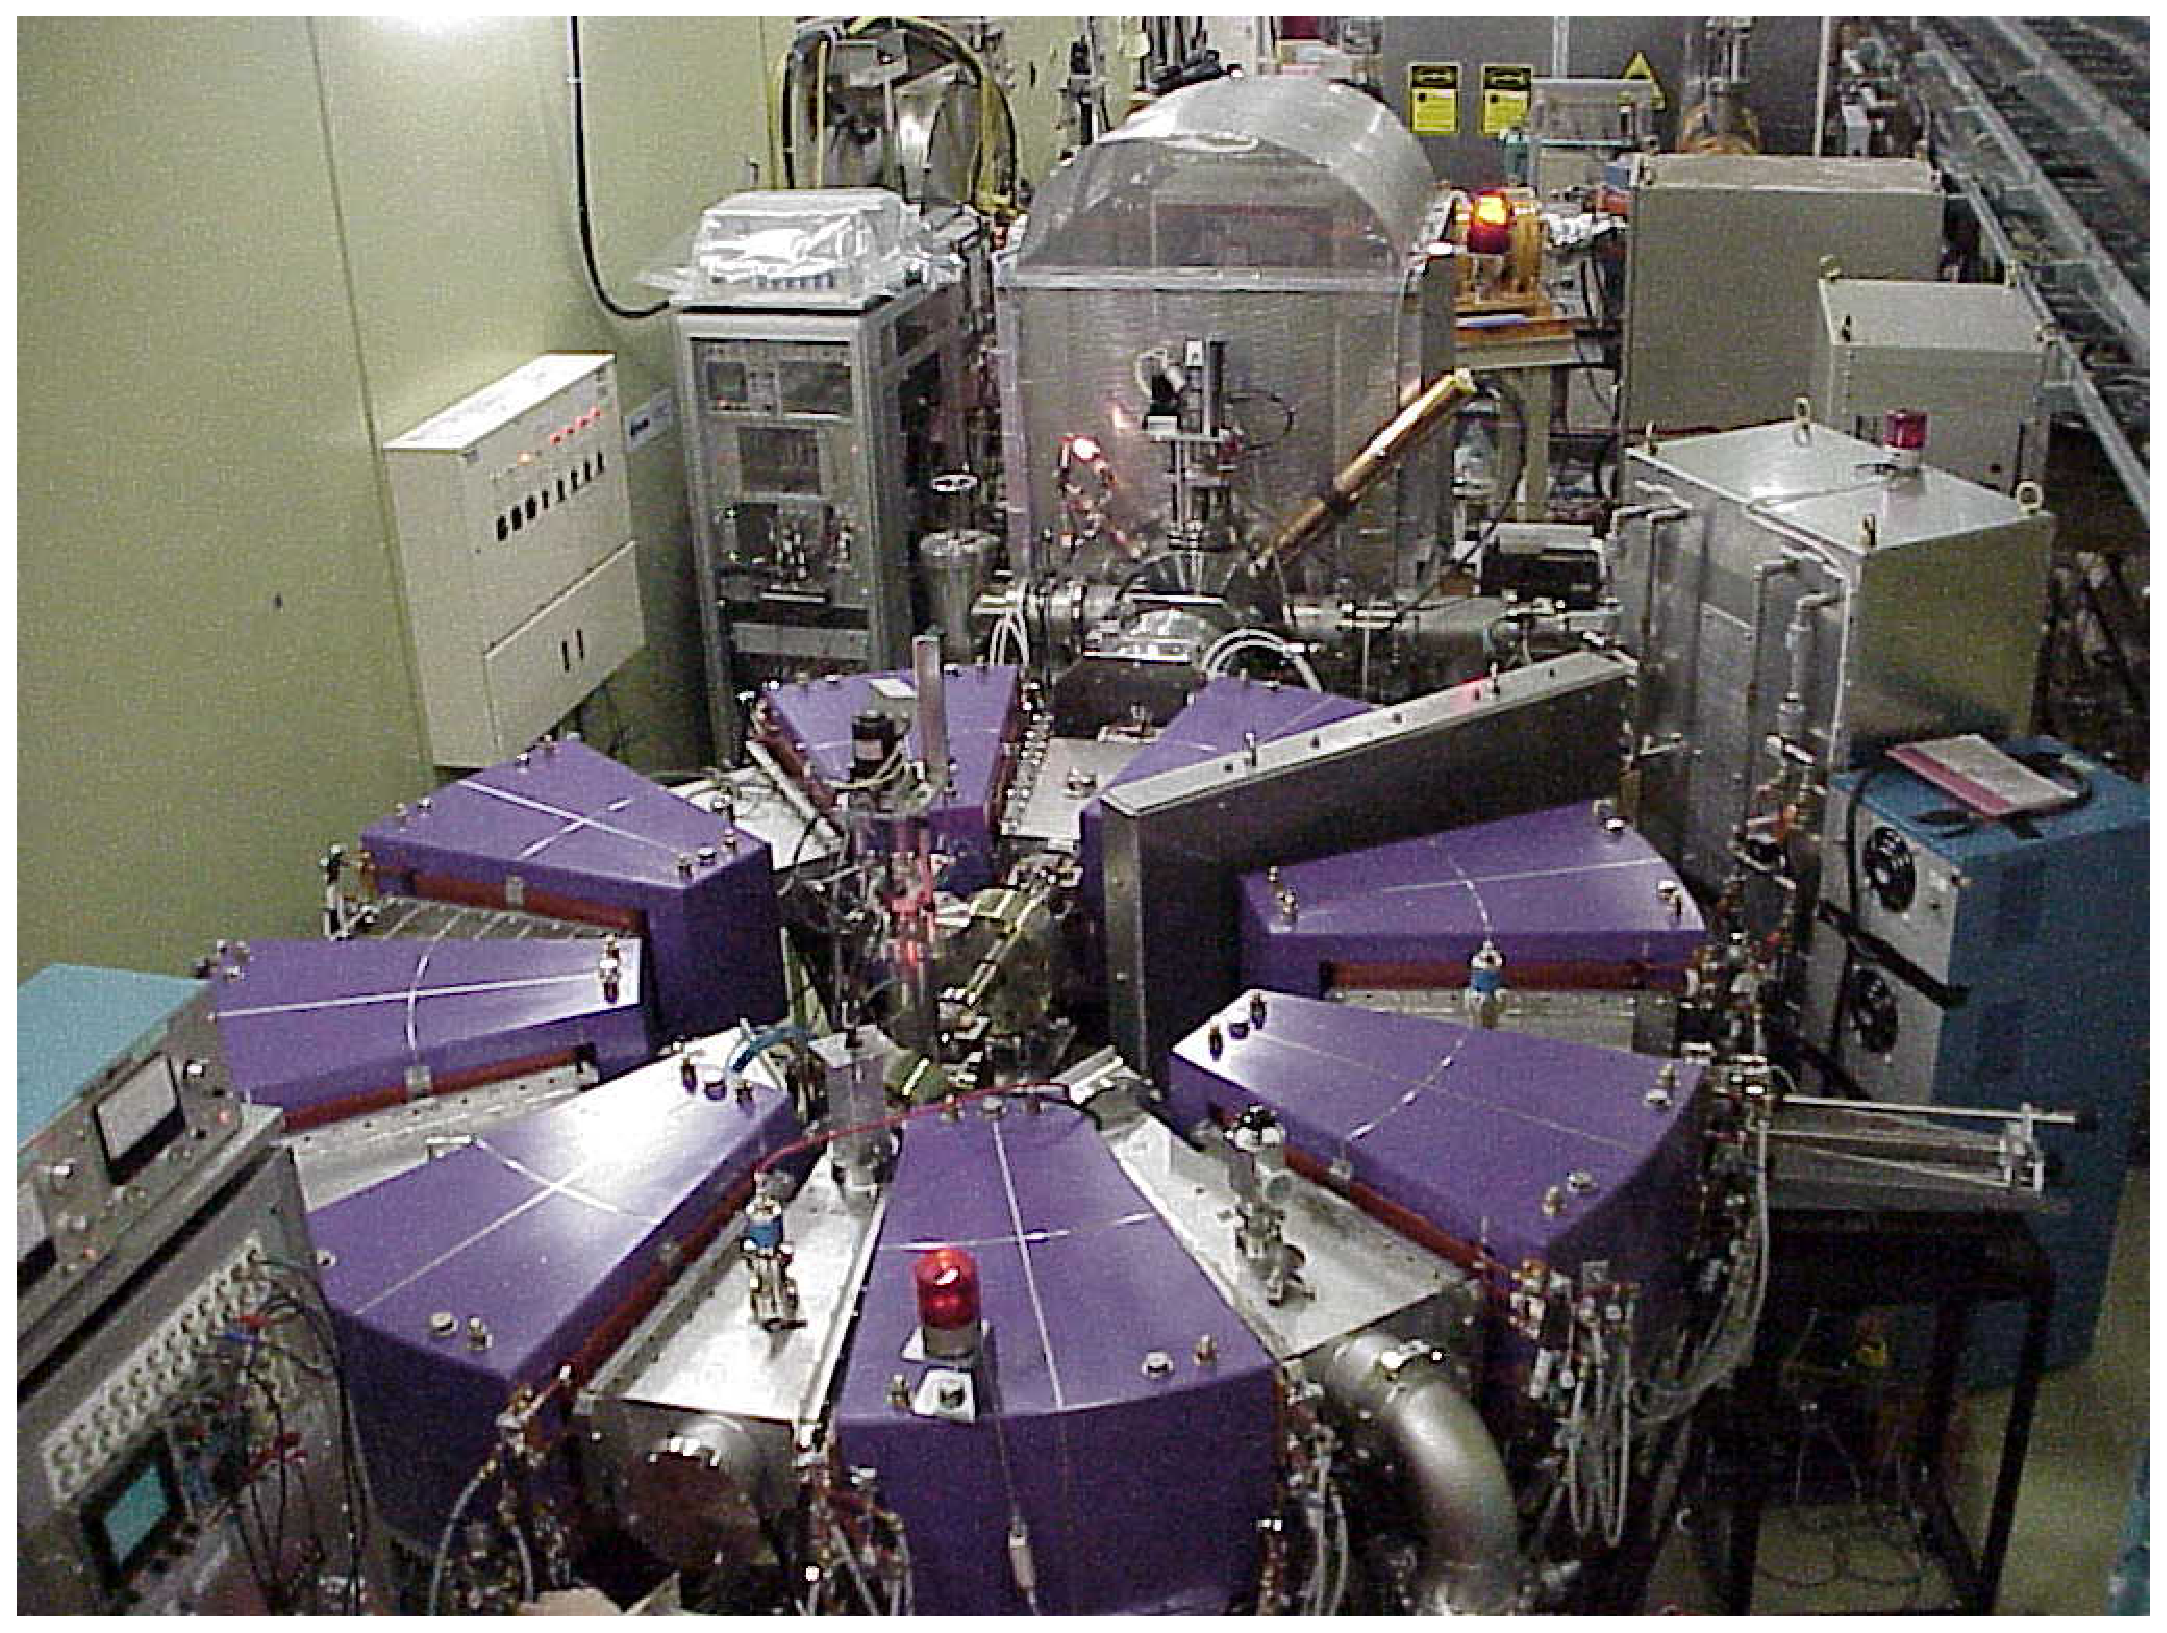
\includegraphics[width=0.99\linewidth,height=2.6cm]{./figures/PoPFFAG.eps}\\
    \includegraphics[width=0.52\linewidth]{./figures/popMagnet.eps}
    \includegraphics[width=0.45\linewidth]{./figures/FFAG31_cavity.eps}
    \caption{
    The first proton FFAG (first beam 1999), particle source 
 in the background, RF system on the right~\cite{BibFFAG-2}. 
    }
    \label{figFFAG_POP}
   \end{minipage}
}
\end{figure}

\section{FFAG Accelerators\label{secFFAG}}

Fixed field alternating gradient accelerators are separated sector ring accelerators 
with fixed-field magnets. Gaps between 
sectors allow the insertion of dedicated equipmnet for injection, acceleration, extraction, etc.
Trajectories spiral under the effect of acceleration (outward as in cyclotrons, 
possibly inward instead, based on particular lattice properties~\cite[FFAGInWardSpiral]). 

FFAGs operate in two ways. Either like synchrotron, using modulated RF and delivering beam pulses,
 or in \textsl{quasi-isochronous} mode, using fixed frequency RF and delivering particle bunches.


\section{Scaling FFAG \label{secCycloClass}}

The scaling FFAG lattice is in general not isochronous (more in Sec.~\ref{SecFFAGQuasiIsoCrhro}), 
by contrast with the cyclotron. This results from a different use of the transverse field index k (Eq.~ref{EqCycloRadialIndex}),
namely, to ensure constant focusing in the former type of lattice, to ensure isochronism in the latter. 




\subsection{Closed orbit, time of flight \label{secCycloClassTra}}

\smallskip
\noindent {\small $\bullet$} Exercise~\ref{secCycloClass}-1 
A FFAG accelerator is a typical case where just putting together drifts and dipoles in a matrix transport 
code won't do. This may at best work for a particular orbit, and will not allow designing the accelerator. 

The common solution os to use a field map, 2- or 3-dimensional. However, mathematical models for the field 
are also a good approach, especially in a preliminary design phase due to the flexibility it brings 
in tayloring the field so to achieve required constrains of orbit excursion limitations, 
focusing, isochronism, etc.

Construct a 45-degree sector mid-plane 2-dimensional field map, with constant vertical field such as to 
achieve a R=0.5~m extraction radius for  10~MeV H- ions (an injector to a higher energy installation, 
typically, with stripping extraction). 
Use a uniform mesh in cylindrical coordinates. 
In a 8-sector configuration (8 times that map, so constituting a complete ring), 
track H- ions on their circular orbit, for a few different momenta ranging from 5~keV to 10~MeV. Plot, 
as a function of momentum, their 
equilibrium orbit radius $R$ and the time of flight $T_{\rm rev}$ on that orbit, 
 from both ray-tracing and  theory on a same graphic. 
Study the effect of the mesh density on the accuracy of trajectory computation. 



\smallskip
\noindent {\small $\bullet$} Exercise~\ref{secCycloClass}-2 
Zgoubi provides analytical models 
 for the magnetic field ${B_y(r,\theta)|_{y=0}}$ in the median plane of a dipole magnet. 
The particular keyword \verb|FFAG| is an instance.  Use it to repoduce the results above. 
From the two series of results, comment on various pros and cons of the two methods, analytical field models and 
fieldmaps.


\subsection{Acceleration}\label{secCycloAccel}


The RF gap provides a voltage  
\begin{equation}
\label{EqRCyclo}
V_{\rm RF}(t) =\hat V \cos ........... 
\end{equation}
Particles are accelerated as long as they belong in the $[-90,+90]$~degree phase interval, 
the closer to $\phi=90$~deg, the smaller the number of turns 
(the time interval) necessary to reach the extraction radius of the FFAG.
A deviation of the field B from the isochronous value $2\pi m f_{\rm rev}/q$
will result in a  shift in the arrival phase of the particle at the RF gap amounting to 
\begin{equation}
\label{EqPFPhaseCyclo}
\Delta (\sin \phi) = 2\pi h n \Delta B/B
\end{equation}

 ******* prendre de valeurs R, B, etc. realistes, e.g. in ../biblio/22047216.pdf, 23001796.pdf*******

\smallskip
\noindent {\small $\bullet$} Exercise~\ref{secCycloAccel}-1 
Assume an accelerating double-gap  configuration as in Fig.~\ref{figLBLCycloSketch}. 
What is the minimum number of turns  expected  from 5~keV to 10~MeV~? Track a particle over that range, 
play with the RF phase, conclude on the  expectations. 
In a V(t) diagram, plot  the position  of the particle along the V(t) curve at the 
accelerating gap, for a magnetic field defect 
$\Delta B/B= 10^{-4}$, homogeneous, in the previous sector  map. 




\subsection{Focusing  \label{secCycloFocus}}

Let $B_r$, $B_y$  be the radial and axial components of the magnetic field, respectively, 
$x=r-R$ a small radial displacement with respect to the reference circular orbit,  
$\omega_{\rm rev} = 2\pi f_{\rm rev} $ the angular frequency of the circular motion. 
The radial and axial  strengths experienced by a particle moving in the vicinity of that reference orbit 
write, to the first order in the radial, $x$,  and axial, $y$, coordinates 
\begin{eqnarray}
\label{EqCycloFoc}
F_x = m \ddot x=  -qvB_y + m\frac{v^2}{r} \approx -q v (B_y|_{x=0} + \frac{\partial B_y}{\partial r}x)  + m\frac{v^2}{R}(1-\frac{x}{R}), & \nonumber \\ 
\textrm{~yielding~}  \ddot x + \omega_r^2 x=0 &  \nonumber \\
F_y= m\ddot y =   qvB_r \approx q v \frac{\partial B_r}{\partial y} y = q v \frac{\partial B_y}{\partial r} y, 
 \textrm{~yielding~}    \ddot{y} - \omega_y^2 y= 0  & ~ ~ ~ 
\end{eqnarray}
wherein 
$\omega_r^2 = \omega_{\rm rev}^2(1+\frac{R}{B}\frac{\partial B_y}{\partial r})$,  
$ \omega_y^2 = \omega_{\rm rev}^2 \frac{R}{B} \frac{\partial B_y}{\partial r}$. 
Focusing by a restoring force appears owing to the use of a magnetic field with radial 
index $k = \frac{R}{B}\frac{\partial B_y}{\partial r}|_{x=0,y=0}$. 
The two quantities 
\begin{equation}
  \nu_r = \omega_r/\omega_{\rm rev} = \sqrt{1+k},   ~ ~ ~ ~ 
 \nu_y=\omega_y /\omega_{\rm rev}  = \sqrt{-k} 
\end{equation}
are known  respectively as the radial and the axial ``wave number'' of 
the oscilatory motion in the neiboring of the reference circular orbit.
Note that $\nu_r^2 + \nu_y^2=1$.
Vertical motion stability requires $k$ to be negative~:  $B_y$ (respectively, the magnet gap) 
is slowly  decreasing (increasing) with radius, restoring force toward the 
median plane. 
Focussing in both radial and axial motions requires $0 < k <-1$, a conditon known as ``weak focusing''.
 Note that  at low energy  the electric field in the 
region of the accelerating gap also contributes to the focusing, an aspect omitted here. 


\smallskip
\noindent {\small $\bullet$} Exercise~\ref{secCycloFocus}-1
Plot two particle trajectories that demonstrate the value of the radial wave number in the uniform 
field of Sec.~\ref{secCycloClass}. Conclude on orbit and horizontal motion  stability. 
Derive the  vertical  transport matrix from ray-tracing, conclude on the stability of the vertical motion
in a uniform field.


\smallskip
\noindent {\small $\bullet$} Exercise~\ref{secCycloFocus}-2
Back to the field map of exercise~\ref{secCycloClass}-1, or to the analytical model 
of exercise~\ref{secCycloClass}-2: introduce a field index $-1<k<0$. 
Plot the radial and vertical phase space of a 5~MeV ion on a $1\mu$m normalized invariant.  
Compute its radial and axial motion wave numbers, $\nu_r$ and $\nu_y$, 
using two different methods, namely, 1-turn mapping and  Fourrier analysis of multi-turn motion. 
From multiturn tracking, generate the envelope of a 5~MeV beam around the ring FFAG.  


\smallskip
\noindent {\small $\bullet$} Exercise~\ref{secCycloFocus}-3
Using either the field map or the analytical model devised in the  exercise~\ref{secCycloFocus}-2, 
 plot the energy dependence of the reference orbit radius, $R(E)$. 
Plot  $\nu_r^2 + \nu_y^2$ as a function of radius, compare with the value of the field index. 
On a common graphic, plot the horizontal phase space of the 1, 10, 20, 50~MeV particle motion,
assuming the latter on a $1\mu$m normalized invariant in each case.
Plot the vertical phase space motion for these very energies. 
Plot the components of the field vector experienced by a particle as a function of 
azimutahl angle, over a few turns.


\subsection{Quasi-isochronous scaling FFAG lattice \label{SecFFAGQuasiIsoCrhro}}

With particular constraints on the field index, 
scaling FFAG lattices can be made \textsl{quasi-isochronous} so allowing the use, as in cyclotrons, of fixed-frequency RF 
for acceleration, with however poor isochronism overcome with brute force RF voltage. 




\section{Non-scaling FFAG \label{secFFAGNS}}



\section{Bibliography}

[BibFFAG-1] MURA, MARKII
O Camelot ??


[BibFFAG-2]
Theme Section: FFAG Accelerators, 
in 
Beam Dynamics Newsletter No. 43, 
Issue Editor C.R. Prior, 
August~2007.




